
\documentclass[xcolor=pdftex,table,11pt]{beamer}
\usetheme{Warsaw}
\usepackage[utf8]{inputenc}
\usepackage[english]{babel}
\usepackage{amsmath}
\usepackage{amsfonts}
\usepackage{amssymb}
\usepackage{multirow}
\usepackage{siunitx}
\usepackage{listings}
\usepackage{tabulary}
\usepackage[highlightcolor=yellow]{../styles/code}
\author{Informática I - Instituto Unviersitario Areonáutico}
\title{Introducción a la programación en C}

\usepackage{booktabs}
\usepackage{longtable}
\newcommand*{\thead}[1]{\multicolumn{1}{c}{\bfseries #1}}

\usepackage{tikz}
\def\checkmark{\tikz\fill[scale=0.3](0,.35) -- (.25,0) -- (1,.7) -- (.25,.15) -- cycle;} 

%\setbeamercovered{transparent} 
%\setbeamertemplate{navigation symbols}{} 
%\logo{} 
%\institute{} 
%\date{} 
%\subject{} 
\begin{document}


\begin{frame}
\titlepage
\end{frame}

\begin{frame}
\tableofcontents
\end{frame}



\begin{frame}{Etapas de un programa en C }

 \begin{enumerate}
   
     	\item<1->  Escritura del código fuente: se pueden utilizar diferentes editores de texto: gedit, VIM, Zinjal, Atom, Emacs, etc. 
     	
\href{https://github.com/danis963/informaticaI_IUA/blob/main/c/c_detras_de_escena/volumen_esfera.c}{\beamergotobutton{Ver en github}}


        \item<2->  Pre-procesamiento: procesa directivas como $\#$include, $\#$define e $\#$if, remueve los comentarios, etc. En general, luego del preprocesamiento, el archivo resultante contiene una gran cantidad de líneas de código.
       
		\href{https://github.com/danis963/informaticaI_IUA/blob/main/c/c_detras_de_escena/volumen_esfera.i}{\beamergotobutton{Ver en github}}
		
		
	\item<3->  Compilado: el compilador de C traduce el código del apartado anterior a assembler. 
     
		\href{https://github.com/danis963/informaticaI_IUA/blob/main/c/c_detras_de_escena/volumen_esfera.s}{\beamergotobutton{Ver en github}}
		
		
				\item<4->  Ensamblado: el ensamblado transforma el programa escrito en lenguaje ensamblador a código objeto. 
		
		\href{https://github.com/danis963/informaticaI_IUA/blob/main/c/c_detras_de_escena/volumen_esfera.o}{\beamergotobutton{Ver en github}}

		

				\item<5->  Enlazado: reune uno o más módulos en código objeto con el código existente en las bibliotecas.
		
		\href{https://github.com/danis963/informaticaI_IUA/blob/main/c/c_detras_de_escena/a.out}{\beamergotobutton{Ver en github}}

   \end{enumerate}
   
   

\end{frame}




\begin{frame}{Buenas practicas de programación}
\begin{itemize}

\item<1-> Proyectos con aproximadamente 300.000 lineas de código o menos
\begin{itemize}
\item<1->  Aplicación promedio para smartphone
\item<2->  Photoshop v1.0 (1990)
\item<3->  Quake 3 (1999)
\item<4->  Transbordador espacial STS (1981)
\end{itemize}

\item<5-> Proyectos con aproximadamente menos de 10 millones de líneas de código
\begin{itemize}
\item<6->  Age of empires - Versión online
\item<7->  Linux kernel 2.2.0
\item<8->  Windows 3.1 (1992)
\end{itemize}


\item<9-> Proyectos con aproximadamente más de 50 millones
\begin{itemize}
\item<10->  Age of empires - Versión online
\item<11->  Linux kernel 2.2.0
\item<12->  Windows 3.1 (1992)
\end{itemize}



\item<13-> Proyectos con aproximadamente más de 2 mil millones de líneas de código
\begin{itemize}
\item<14->  Google Internet Services
\end{itemize}


\end{itemize}



\end{frame}



\begin{frame}{Buenas practicas de programación: reglas de estilo}
\begin{itemize}
\item<1-> Variables 
	\begin{itemize}
		\item<2-> Los nombres deben ser cortos, descriptivos y concretos
		\item<3-> Si el nombre contiene dos o más palabras, se las debe separar por \_
		\item<4-> Deben inicializarse a un valor conocido al momento de la declaración
	\end{itemize}
	
\item<5-> Constantes definidas con \# define 
	\begin{itemize}
		\item<6-> Su identificador debe escribirse con mayúsculas
	\end{itemize}



\item<7-> Indentación del código
	\begin{itemize}
		\item<8-> Debe realizarse con tabulaciones, nunca con espacios
		\item<9-> Deben colocarse llaves para demarcar gráficamente el código que ejcutará cada estructura

		\item<10-> Las llaves deben escribirse siempre
		
		\item<11-> Las líneas de código no deben superar la longitud de 80 caracteres

		
	\end{itemize}

\item<12-> Instrucciones que se deben evitar
	\begin{itemize}
		\item<13-> goto
		\item<14-> Break
		\item<15-> Continue

		
	\end{itemize}

\end{itemize}

    
\end{frame}






\begin{frame} {Tipos de datos en C}
El lenguaje de programación C es \textbf{fuertemente tipado}, es decir que cada vez que se necesite declarar u operar con una variable, se debe definir y tener presente el tipo de la misma. \\
Nota: ver los tipos de datos \textit{Unsigned}
\begin{table}
\begin{tabular}{l | c | c | c | l }
Tipo de dato & Descripción & Rango  \\
\hline \hline
short & Valor entero de 2 bytes & $-2^{16}$ a $2^{16} -1 $\\ 
int & 	Valor entero de 4 bytes & $-2^{32}$ a $2^{32} -1 $\\ 
long & 	Valor entero de 8 bytes & $-2^{64}$ a $2^{64} -1 $\\ 
char & Caracteres ASCII & $-128 $ a $127$\\ 
float & Valor decimal de 4 bytes & $\num{3.4e-38} $ a $\num{3.4e-38}$\\ 
double & Valor decimal de 8 bytes & $\num{1.7e-308} $ a $\num{1.7e-308}$\\ 
bool & Valor binario &True o False\\ 
void & Tipo de dato nulo &\\ 
 string & Cadena de char  &\\ 
\end{tabular}
\caption{Tipos de datos en C}

\end{table}

\end{frame}


\begin{frame}[allowframebreaks] {Entrada y salida de datos}
Para imprimir por pantalla o ingresar datos a un programa en C, se debe informar \textbf{expresamente} el tipo de dato que se espera imprimir y/o recibir.
Esto se realiza mediante el uso de \textbf{especificadores de formato}.

\begin{table}
\begin{tabular}{l | c | l }
Tipo de dato & Especificador de formato \\
\hline \hline
short & $\%hd$ \\ 
int & 	$\%d$ \\ 
long & 	$\%li$ \\ 
char & $\%c$\\ 
float & $\%f$ \\ 
double & $\%lf$\\ 
\end{tabular}
\caption{Especificadores de formato en C}
\end{table}
 \begin{block}{Scanf}
Es una función de la librería de entrada/salida de C que permite tomar información desde el teclado.\\ 

Sintaxis: scanf("especificador de formato", $\&$variable); \\ 
Ejemplo	: scanf("$\%d$", $\&$edad); \\ 
    \end{block}

 \begin{block}{Printf}
Es una función de la librería de entrada/salida de C que permite imprimir información por pantalla.\\ 
Sintaxis: printf("especificador de formato", variable); \\ 
Ejemplo: printf("Su edad es: " $\%d$ , edad);
    \end{block}
    
Nota: para estos ejemplos se supone que la variable se ha declarado de tipo int. Ver ejemplos siguientes.
\codesetstylefrombeamer
\cppfile{../../c/src/1-0_data_types_edad_peso.c}
\end{frame}





\begin{frame}[allowframebreaks] {Operadores en C}

Operadores de asignación:

\begin{table}
\begin{tabular}{p{15mm} | p{35mm} | p{22mm} | p{22mm} | p{22mm} }
Operador & Acción & Ejemplo & Resultado\\
\hline \hline 
= & 	Asignación básica  		  & $x=10$ 	 	& x vale 10\\
*= 	& 	Asignación producto       & $x*=10$ 	& x vale 100 \\
/= 	& 	Asignación división       & $x/=2$      & x vale 50 \\
+= 		& Asignación suma         & $x+=5$  	& x vale 55\\
-= 			& 	Asignación resta  & $x-=7$  	& x vale 48\\ 

\end{tabular}
\caption{Operadores de asignación}
\end{table}



\newpage
Operadores aritméticos:

\begin{table}
\begin{tabular}{p{15mm} | p{35mm} | p{22mm} | p{22mm} | p{22mm} }
Operador & Acción & Ejemplo & Resultado\\
\hline \hline  
- 	& 	Resta & $x=12 - 3 $ & x vale 9\\
+ 	& 	Suma & $x=12 + 3 $ & x vale 15\\
* 	& 	Multiplicación &  $x=12 * 3 $ & x vale 36\\
/ 	& 	División &  $x=12 / 3 $ & x vale 4\\
--	& 	Decremento &  $x=12; x-- $ & x vale 11\\
++	& 	Incremento &  $x=12; x++ $ & x vale 13\\
\%	& 	Modulo &  $x=13 \% 2 $ & x vale 1\\
\end{tabular}
\caption{Operadores de asignación}
\end{table}



\end{frame}


\begin{frame}{Precedencia de operadores}
El lenguaje C evalúa las expresiones aritméticas en una secuencia precisa, por lo general son las mismas que aplicaríamos en el álgebra:\\

\begin{enumerate}
\item<1->  Las operaciones de multiplicación, división y módulo se resuelven primero. Si en una misma operación aparecen varias de ellas, se resuelven de izquierda a derecha

\item<2->  Las operaciones de suma y resta se aplican después. Si hubiese varias de estas, C separará en términos al igual que se haría en el álgebra

\item<3-> Luego de resueltas todas las operaciones, se procede a la asignación

\end{enumerate}
\end{frame}

\begin{frame}{Precedencia de operadores: ejemplo}


 \begin{block}{Ecuación de una recta en forma algebraica}
\begin{equation}
y(x) = a x + b
\end{equation}
    \end{block}
    

 \begin{block}{Ecuación de una recta en C}
\begin{equation}
y = a * x + b
\end{equation}


  \end{block}

 \begin{block}{Precedencia de operadores}
 \begin{enumerate}
\item<1->  Operación $a * x$
\item<2->  Operación $+b$
\item<3->  Asignación del resultado a la variable $y$
\end{enumerate}
  \end{block}
\end{frame}
\begin{frame}{Precedencia de operadores: ejemplo en C}
\codesetstylefrombeamer
\cppfile{../../c/src/1-1_presedencia_operadores.c}
\end{frame}

\begin{frame}{Estrucutra selectiva múltiple: Switch}

 \begin{block}{Aplicación}
 Permite que un programa en C tome diferentes caminos en función del valor que tome una determinada instrucción.
 
 
 \end{block}

 \begin{block}{Pseudocódigo}

    \begin{itemize}
   \item[]Según sea (variable de control)
   \begin{itemize}

     	\item[] Caso 1:
     	    \begin{itemize}
     			\item[] Instrucciones caso 1
     			\item[] Instrucciones caso 1
     			\item[] frenar
     		   \end{itemize}

        \item[] Caso 2:
     	    \begin{itemize}
     			\item[] Instrucciones caso 2
     			\item[] Instrucciones caso 2

     			\item[] frenar
 		
   			\end{itemize}
    
    \item[] Caso por descarte:
     	    \begin{itemize}
     			\item[] Instrucciones caso por descarte
     			\item[] frenar
 		
   			\end{itemize}

   \end{itemize}

	\end{itemize}

 \end{block}





\end{frame}



\begin{frame}{Estrucutra selectiva múltiple: Switch}

\begin{figure}

\includegraphics[scale=0.201]{../img/exported/switch.png}
\caption{Diagrama de flujo para la estructura switch}
\end{figure}
\end{frame}


\begin{frame}{Estrucutra selectiva múltiple: Switch}
\codesetstylefrombeamer
\cppfile{../../c/src/1-2_switch_case.c}
\end{frame}


\begin{frame}{Estrucutra selectiva múltiple: Switch - ejemplos}
 \begin{enumerate}
   
     	\item Diseñar y codificar un programa que permita simular una calculadora de numeros enteros.
     	Luego de recibir dos operandos enteros, se deben poder realizar las siguientes opciones:
     	 \begin{enumerate}
     	 \item Sumar
		 \item Restar
		\item Multiplicar
		\item Dividir
	   	Si el usuario ingresa una opción inválida, esta debe ser informada.
     	 \end{enumerate}

\href{https://github.com/danis963/informaticaI_IUA/blob/main/c/src/1-3_switch_case_calculadora.c}{\beamergotobutton{Ver en github}}



     	\item Diseñar y codificar un programa que permita conocer el estado de un alumno en función de la nota de su parcial. Si la nota ingresada es menor a cuatro, se debe imprimir reprobado. Entre cuatro y diez, aprobado. Cualquier otra opción, imrpimir mensaje indicano que la nota es incorrecta. Se debe usar una estructura selectiva switch.
     	
	\href{https://github.com/danis963/informaticaI_IUA/blob/main/c/src/1-3_switch_case_notas.c}{\beamergotobutton{Ver en github}}

   
   \end{enumerate}
   

\end{frame}





\begin{frame}{Operadores relacionales}
\begin{block}{}
Los operadores relacionales comparan el primer operando con el segundo y prueban la validez de la relación expresada. El resultado de una operación relacional es siempre verdadero o falso.
\end{block}



\begin{table}
\begin{tabular}{l | c | l }
Operador & Relación \\
\hline \hline
$<$ & Primer operando menor que el segundo operando \\ 
$>$ & 	Primer operando mayor que el segundo operando\\ 
$<=$ & 	Primer operando menor o igual que segundo operando \\ 
$>=$ & Primer operando mayor o igual que segundo operando \\ 
$==$ & Primer operando igual a segundo operando \\ 
$!=$ & Primer operando no igual a segundo operando\\ 
\end{tabular}
\caption{Operadores relacionales en C}
\end{table}


\end{frame}


\begin{frame}{Operadores lógicos}
\begin{block}{}
Los operadores lógicos proporcionan un resultado a partir de que se cumpla o no una cierta condición. Sus operandos y su resultado son valores booleanos (verdadero o falso).
\end{block}



\begin{table}
\begin{tabular}{l | c}
Operador & Relación \\
\hline \hline
$\&\&$ &  operador AND (y) lógico \\ 
$||$ & 	operador OR  (o) lógico\\ 
$!=$ & 	Operador NOT (no) lógico \\ 
\end{tabular}
\caption{Operadores lógicos en C}
\end{table}

\end{frame}


\begin{frame}{Estructura selectiva simple: Diagrama de flujo}
\begin{block}{Definición}
Se definen un conjunto de acciones a realizar, sólo si la condición de evaluación resulta VERDADERA. Para el caso contrario, no se realiza ninguna acción. 
\end{block}


 \begin{figure}
 \centering
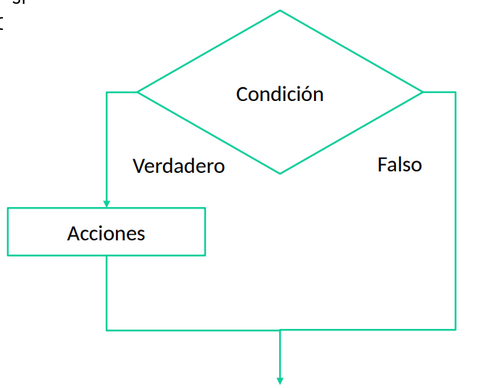
\includegraphics[scale=0.3]{../img/exported/if.png}
\caption{Diagrama de flujo estructura selectiva simple}
\end{figure}

\end{frame}


\begin{frame}{Estructura selectiva simple: pseudocódigo}
\begin{block}{Definición}
Se definen un conjunto de acciones a realizar, sólo si la condición de evaluación resulta VERDADERA. Para el caso contrario, no se realiza ninguna acción. 
\end{block}

 \begin{itemize}
   \item[]<1-> Inicio del algoritmo

   \begin{itemize}
   
     	\item[]<2-> si (condición es verdadera)
     	\begin{itemize}
     			\item[]<3->  acción 1;
     			\item[]<4->  acción 2;
     			\item[]<5->  acción 3;
     			\item[]<6->  acción 4;
     	\end{itemize}
     	 
   \end{itemize}
  \item[]<7-> Fin del algoritmo
\end{itemize}

\end{frame}



\begin{frame}{Estructura selectiva simple: Ejemplo en C}
\codesetstylefrombeamer
\cppfile{../../c/src/2-0_if.c}
\end{frame}



\begin{frame}{Estructura selectiva doble: Diagrama de flujo}
\begin{block}{Definición}
Se definen un conjunto de acciones a realizar para el caso en que la condición dentro del rombo de decisión de la figura sea verdadera, como así también para el caso contrario. Es decir, la condición en el rombo de decisión resulte falsa.
\end{block}


 \begin{figure}
 \centering
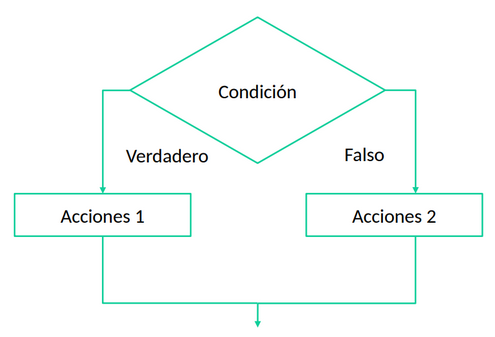
\includegraphics[scale=0.3]{../img/exported/if_else.png}
\caption{Diagrama de flujo estructura selectiva doble}
\end{figure}

\end{frame}


\begin{frame}{Estructura selectiva doble: pseudocódigo}
\begin{block}{Definición}
Se definen un conjunto de acciones a realizar para el caso en que la condición dentro del rombo de decisión de la figura sea verdadera, como así también para el caso contrario. Es decir, la condición en el rombo de decisión resulte falsa.
\end{block}

 \begin{itemize}
   \item[]<1-> Inicio del algoritmo

   \begin{itemize}
   
     	\item[]<2-> si (condición es verdadera)
     	\begin{itemize}
     			\item[]<3->  acción 1;
     			\item[]<4->  acción 2;
     			\item[]<5->  acción 3;
     			\item[]<6->  acción 4;
     	\end{itemize}
          	\item[]<7-> si no (condición falsa)
     	\begin{itemize}
     			\item[]<8->  acción 1;
     			\item[]<9->  acción 2;
     			\item[]<10->  acción 3;
     			\item[]<11->  acción 4;
     	\end{itemize}
   \end{itemize}
  \item[]<12-> Fin del algoritmo
\end{itemize}

\end{frame}



\begin{frame}{Estructura selectiva doble: Ejemplo en C}
\codesetstylefrombeamer
\cppfile{../../c/src/2-1_if_else.c}
\end{frame}


\begin{frame}{Estructura selectiva doble: ejemplos}
 \begin{enumerate}
   
     	\item Diseñar y codificar un programa que tome un número entero por teclado e indique si el número es positivo, negativo o cero.     	
\href{https://github.com/danis963/informaticaI_IUA/blob/main/c/src/2-2_if_else.c}{\beamergotobutton{Ver en github}}



     	\item Diseñar y codificar un programa que tome dos números enteros por teclado e indique cual es el mayor. Si los números son iguales, se debe informar esta condición.
     	
	\href{https://github.com/danis963/informaticaI_IUA/blob/main/c/src/2-3_if_else.c}{\beamergotobutton{Ver en github}}

     	\item Diseñar y codificar un programa que tome las coordenadas de un punto en el plano cartesiano (x;y) e imprima por pantalla a que cuadrante pertenece el punto.


	\href{https://github.com/danis963/informaticaI_IUA/blob/main/c/src/2-4_if_else.c}{\beamergotobutton{Ver en github}}
   
   
   
       \item Diseñar y codificar un programa que tome por teclado el valor de cada uno de los lados de un triángulo y determine si es equilátero, isosceles o escaleno. También debe imprimir el perímetro del mismo.


	\href{https://github.com/danis963/informaticaI_IUA/blob/main/c/src/2-5_if_else.c}{\beamergotobutton{Ver en github}}
   \end{enumerate}
   

\end{frame}

\begin{frame}{Ciclo repetitivo for}

\begin{block}{Definición}
Es una estructura repetitiva controlada por contador. En general, se la utiliza cuando se conoce previamente la cantida de veces que las acciones seran ejecutadas.
\end{block}

Esta compuesto por:

\begin{itemize}
\item Valor inicial de la variable de control
\item Condicion de continuacion de ciclo
\item Incremento de la variable de control
\end{itemize}

\end{frame}


\begin{frame}{Ciclo repetitivo for: pseudocodigo y diagrama de flujo }

\begin{itemize}
   \item[]<1-> Inicio del algoritmo

   \begin{itemize}
   		\item[]<2-> i=0 definicion de la variable control
     	anidacion\item[]<3-> Para i=0 hasta N
     	\begin{itemize}
     			\item[]<4->  acción 1;
     			\item[]<5->  acción 2;
     			\item[]<6->  acción 3;
     			\item[]<7->  acción 4;
     	\end{itemize}
   \end{itemize}
  \item[]<8-> Fin del algoritmo
  \item[]<9-> 
   \begin{figure}
 \centering
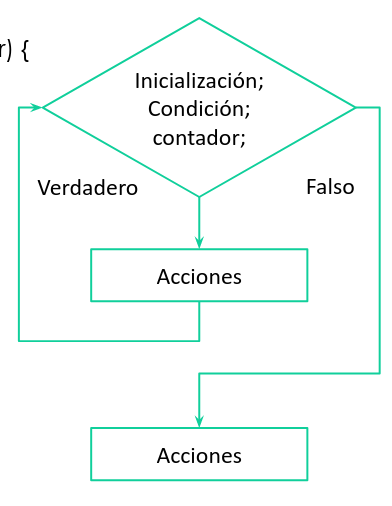
\includegraphics[scale=0.25]{../img/exported/for.png}
\caption{Estructura repetitiva For.}
\end{figure}
\end{itemize}
\end{frame}




\begin{frame}{Ciclo repetitivo for: Codificacion en C}
\codesetstylefrombeamer
\cppfile{../../c/src/3-0-for.c}
\end{frame}


\begin{frame}[allowframebreaks]{Ciclo repetitivo for: Tabla de verificación}

\begin{columns}
\column{0.5\textwidth}
\begin{tabular}{|c|c|c|c|}
\hline 
ii &ii $<5$ & printf("\%d",i) & ii++ \\ 
\hline 
0 &  &  &  \\ 
\hline 
\end{tabular} 
\column{0.3\textwidth}
 \begin{figure}
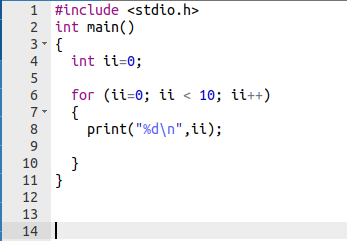
\includegraphics[scale=0.4]{../img/exported/for_code.png}
\caption{Estructura repetitiva for: ejemplo}
\end{figure}
\end{columns}


\begin{columns}
\column{0.5\textwidth}
\begin{tabular}{|c|c|c|c|}
\hline 
ii &ii $<$5 & printf("\%d",i) & ii++ \\ 
\hline 
0 & \checkmark &  &  \\ 
\hline 
\end{tabular} 
\column{0.3\textwidth}
 \begin{figure}
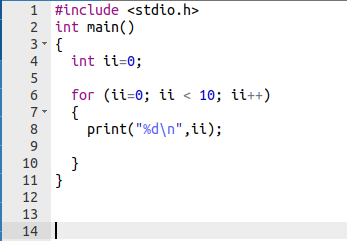
\includegraphics[scale=0.4]{../img/exported/for_code.png}
\caption{Estructura repetitiva for: ejemplo}
\end{figure}
\end{columns}

\begin{columns}
\column{0.5\textwidth}
\begin{tabular}{|c|c|c|c|}
\hline 
ii &ii $<$5 & printf("\%d",i) & ii++ \\ 
\hline 
0 & \checkmark & 0 &  \\ 
\hline 
\end{tabular} 
\column{0.3\textwidth}
 \begin{figure}
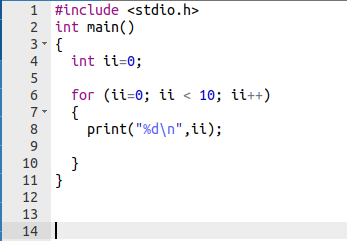
\includegraphics[scale=0.4]{../img/exported/for_code.png}
\caption{Estructura repetitiva for: ejemplo}
\end{figure}
\end{columns}

\begin{columns}
\column{0.5\textwidth}
\begin{tabular}{|c|c|c|c|}
\hline 
ii &ii $<$5 & printf("\%d",i) & ii++ \\ 
\hline 
0 & \checkmark & 0 & 1\\ 
\hline 
\end{tabular} 
\column{0.3\textwidth}
 \begin{figure}
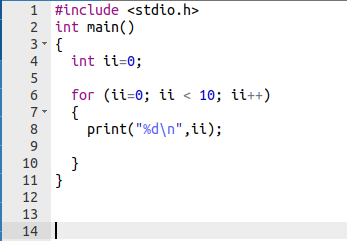
\includegraphics[scale=0.4]{../img/exported/for_code.png}
\caption{Estructura repetitiva for: ejemplo}
\end{figure}
\end{columns}




\begin{columns}
\column{0.5\textwidth}
\begin{tabular}{|c|c|c|c|}
\hline 
ii &ii $<$5 & printf("\%d",i) & ii++ \\ 
\hline 
0 & \checkmark & 0 & 1\\ 
\hline 
1 & & &\\ 
\hline
\end{tabular} 
\column{0.3\textwidth}
 \begin{figure}
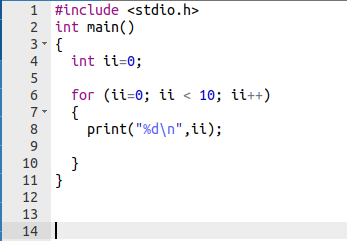
\includegraphics[scale=0.4]{../img/exported/for_code.png}
\caption{Estructura repetitiva for: ejemplo}
\end{figure}
\end{columns}

\begin{columns}
\column{0.5\textwidth}
\begin{tabular}{|c|c|c|c|}
\hline 
ii &ii $<$5 & printf("\%d",i) & ii++ \\ 
\hline 
0 & \checkmark & 0 & 1\\ 
\hline 
1 & \checkmark & 1 &\\ 
\hline 
\end{tabular} 
\column{0.3\textwidth}
 \begin{figure}
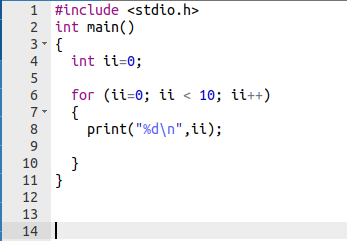
\includegraphics[scale=0.4]{../img/exported/for_code.png}
\caption{Estructura repetitiva for: ejemplo}
\end{figure}
\end{columns}

\begin{columns}
\column{0.5\textwidth}
\begin{tabular}{|c|c|c|c|}
\hline 
ii &ii $<$5 & printf("\%d",i) & ii++ \\ 
\hline 
0 & \checkmark & 0 & 1\\ 
\hline 
1 & \checkmark & 1 &\\ 
\hline 
\end{tabular} 
\column{0.3\textwidth}
 \begin{figure}
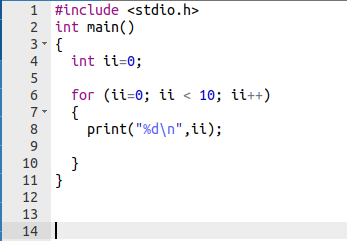
\includegraphics[scale=0.4]{../img/exported/for_code.png}
\caption{Estructura repetitiva for: ejemplo}
\end{figure}
\end{columns}


\begin{columns}
\column{0.5\textwidth}
\begin{tabular}{|c|c|c|c|}
\hline 
ii &ii $<$5 & printf("\%d",i) & ii++ \\ 
\hline 
0 & \checkmark & 0 & 1\\ 
\hline 
1 & \checkmark & 1 & 2 \\ 
\hline 
\end{tabular} 
\column{0.3\textwidth}
 \begin{figure}
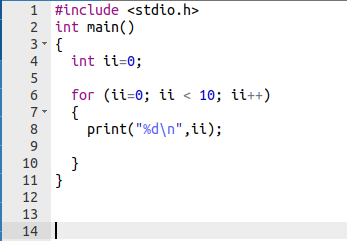
\includegraphics[scale=0.4]{../img/exported/for_code.png}
\caption{Estructura repetitiva for: ejemplo}
\end{figure}
\end{columns}



\begin{columns}
\column{0.5\textwidth}
\begin{tabular}{|c|c|c|c|}
\hline 
ii &ii $<$5 & printf("\%d",i) & ii++ \\ 
\hline 
0 & \checkmark & 0 & 1\\ 
\hline 
1 & \checkmark & 1 & 2 \\ 
\hline 
2 &  &  &  \\ 
\hline 
\end{tabular} 
\column{0.3\textwidth}
 \begin{figure}
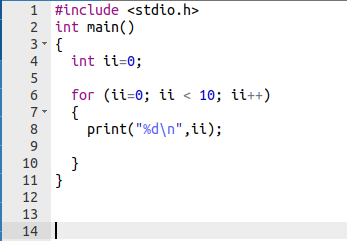
\includegraphics[scale=0.4]{../img/exported/for_code.png}
\caption{Estructura repetitiva for: ejemplo}
\end{figure}
\end{columns}



\begin{columns}
\column{0.5\textwidth}
\begin{tabular}{|c|c|c|c|}
\hline 
ii &ii $<$5 & printf("\%d",i) & ii++ \\ 
\hline  
0 & \checkmark & 0 & 1\\ 
\hline 
1 & \checkmark & 1 & 2 \\ 
\hline 
2 & \checkmark &  &  \\ 
\hline 
\end{tabular} 
\column{0.3\textwidth}
 \begin{figure}
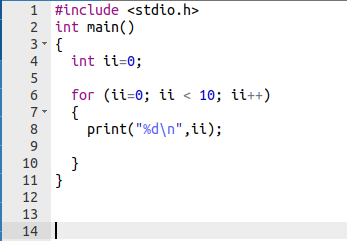
\includegraphics[scale=0.4]{../img/exported/for_code.png}
\caption{Estructura repetitiva for: ejemplo}
\end{figure}
\end{columns}

\begin{columns}
\column{0.5\textwidth}
\begin{tabular}{|c|c|c|c|}
\hline 
ii &ii $<$5 & printf("\%d",i) & ii++ \\ 
\hline 
0 & \checkmark & 0 & 1\\ 
\hline 
1 & \checkmark & 1 & 2 \\ 
\hline 
2 & \checkmark & 2 &  \\ 
\hline 
\end{tabular} 
\column{0.3\textwidth}
 \begin{figure}
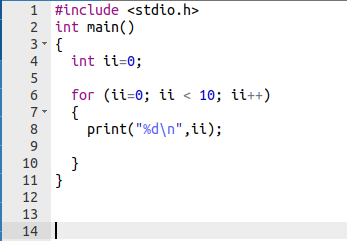
\includegraphics[scale=0.4]{../img/exported/for_code.png}
\caption{Estructura repetitiva for: ejemplo}
\end{figure}
\end{columns}




\begin{columns}
\column{0.5\textwidth}
\begin{tabular}{|c|c|c|c|}
\hline 
ii &ii $<$5 & printf("\%d",i) & ii++ \\ 
\hline 
0 & \checkmark & 0 & 1\\ 
\hline 
1 & \checkmark & 1 & 2 \\ 
\hline 
2 & \checkmark & 2 & 3 \\ 
\hline 
\end{tabular} 
\column{0.3\textwidth}
 \begin{figure}
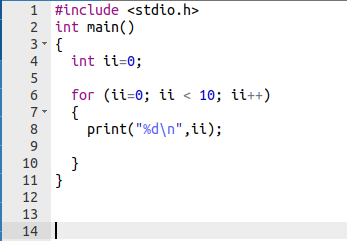
\includegraphics[scale=0.4]{../img/exported/for_code.png}
\caption{Estructura repetitiva for: ejemplo}
\end{figure}
\end{columns}

\begin{columns}
\column{0.5\textwidth}
\begin{tabular}{|c|c|c|c|}
\hline 
ii &ii $<$5 & printf("\%d",i) & ii++ \\ 
\hline 
0 & \checkmark & 0 & 1\\ 
\hline 
1 & \checkmark & 1 & 2 \\ 
\hline 
2 & \checkmark & 2 & 3 \\ 
\hline 
3 & & & \\ 
\hline 
\end{tabular} 
\column{0.3\textwidth}
 \begin{figure}
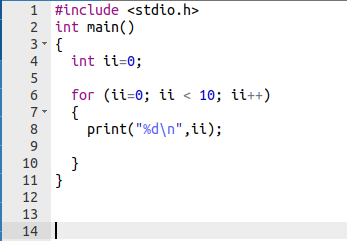
\includegraphics[scale=0.4]{../img/exported/for_code.png}
\caption{Estructura repetitiva for: ejemplo}
\end{figure}
\end{columns}


\begin{columns}
\column{0.5\textwidth}
\begin{tabular}{|c|c|c|c|}
\hline 
ii &ii $<$5 & printf("\%d",i) & ii++ \\ 
\hline 
0 & \checkmark & 0 & 1\\ 
\hline 
1 & \checkmark & 1 & 2 \\ 
\hline 
2 & \checkmark & 2 & 3 \\ 
\hline 
3 & \checkmark  & & \\ 
\hline 
\end{tabular} 
\column{0.3\textwidth}
 \begin{figure}
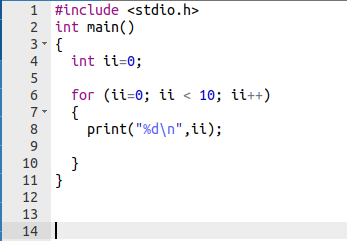
\includegraphics[scale=0.4]{../img/exported/for_code.png}
\caption{Estructura repetitiva for: ejemplo}
\end{figure}
\end{columns}


\begin{columns}
\column{0.5\textwidth}
\begin{tabular}{|c|c|c|c|}
\hline 
ii &ii $<$5 & printf("\%d",i) & ii++ \\ 
\hline 
0 & \checkmark & 0 & 1\\ 
\hline 
1 & \checkmark & 1 & 2 \\ 
\hline 
2 & \checkmark & 2 & 3 \\ 
\hline 
3 & \checkmark  & 3 & \\ 
\hline 
\end{tabular} 
\column{0.3\textwidth}
 \begin{figure}
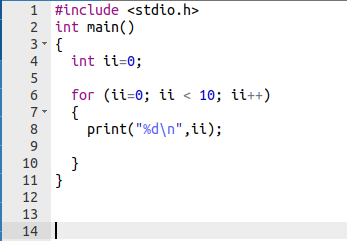
\includegraphics[scale=0.4]{../img/exported/for_code.png}
\caption{Estructura repetitiva for: ejemplo}
\end{figure}
\end{columns}

\begin{columns}
\column{0.5\textwidth}
\begin{tabular}{|c|c|c|c|}
\hline 
ii &ii $<$5 & printf("\%d",i) & ii++ \\ 
\hline 
0 & \checkmark & 0 & 1\\ 
\hline 
1 & \checkmark & 1 & 2 \\ 
\hline 
2 & \checkmark & 2 & 3 \\ 
\hline 
3 & \checkmark  & 3 & 4 \\ 
\hline 
\end{tabular} 
\column{0.3\textwidth}
 \begin{figure}
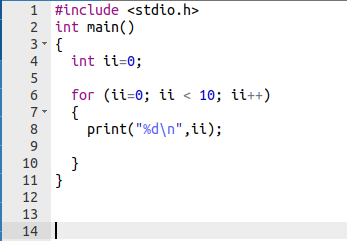
\includegraphics[scale=0.4]{../img/exported/for_code.png}
\caption{Estructura repetitiva for: ejemplo}
\end{figure}
\end{columns}

\begin{columns}
\column{0.5\textwidth}
\begin{tabular}{|c|c|c|c|}
\hline 
ii &ii $<$5 & printf("\%d",i) & ii++ \\ 
\hline 
0 & \checkmark & 0 & 1\\ 
\hline 
1 & \checkmark & 1 & 2 \\ 
\hline 
2 & \checkmark & 2 & 3 \\ 
\hline 
3 & \checkmark  & 3 & 4 \\ 
\hline 
4 & &  &  \\ 
\hline 
\end{tabular} 
\column{0.3\textwidth}
 \begin{figure}
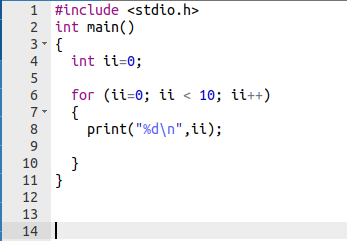
\includegraphics[scale=0.4]{../img/exported/for_code.png}
\caption{Estructura repetitiva for: ejemplo}
\end{figure}
\end{columns}


\begin{columns}
\column{0.5\textwidth}
\begin{tabular}{|c|c|c|c|}
\hline 
ii &ii $<$5 & printf("\%d",i) & ii++ \\ 
\hline 
0 & \checkmark & 0 & 1\\ 
\hline 
1 & \checkmark & 1 & 2 \\ 
\hline 
2 & \checkmark & 2 & 3 \\ 
\hline 
3 & \checkmark  & 3 & 4 \\ 
\hline 
4 & \checkmark &  &  \\ 
\hline 
\end{tabular} 
\column{0.3\textwidth}
 \begin{figure}
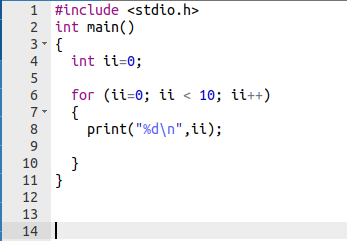
\includegraphics[scale=0.4]{../img/exported/for_code.png}
\caption{Estructura repetitiva for: ejemplo}
\end{figure}
\end{columns}

\begin{columns}
\column{0.5\textwidth}
\begin{tabular}{|c|c|c|c|}
\hline 
ii &ii $<$5 & printf("\%d",i) & ii++ \\ 
\hline 
0 & \checkmark & 0 & 1\\ 
\hline 
1 & \checkmark & 1 & 2 \\ 
\hline 
2 & \checkmark & 2 & 3 \\ 
\hline 
3 & \checkmark  & 3 & 4 \\ 
\hline 
4 & \checkmark & 4 &  \\ 
\hline 
\end{tabular} 
\column{0.3\textwidth}
 \begin{figure}
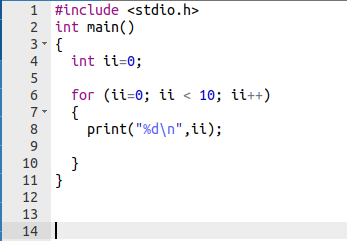
\includegraphics[scale=0.4]{../img/exported/for_code.png}
\caption{Estructura repetitiva for: ejemplo}
\end{figure}
\end{columns}




\begin{columns}
\column{0.5\textwidth}
\begin{tabular}{|c|c|c|c|}
\hline 
ii &ii $<$5 & printf("\%d",i) & ii++ \\ 
\hline 
0 & \checkmark & 0 & 1\\ 
\hline 
1 & \checkmark & 1 & 2 \\ 
\hline 
2 & \checkmark & 2 & 3 \\ 
\hline 
3 & \checkmark  & 3 & 4 \\ 
\hline 
4 & \checkmark & 4 & 5 \\ 
\hline 
\end{tabular} 
\column{0.3\textwidth}
 \begin{figure}
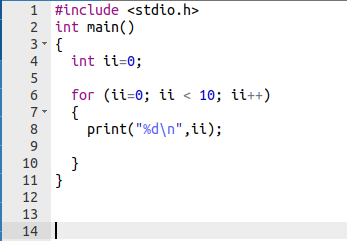
\includegraphics[scale=0.4]{../img/exported/for_code.png}
\caption{Estructura repetitiva for: ejemplo}
\end{figure}
\end{columns}

\begin{columns}
\column{0.5\textwidth}
\begin{tabular}{|c|c|c|c|}
\hline 
ii &ii $<$5 & printf("\%d",i) & ii++ \\ 
\hline 
0 & \checkmark & 0 & 1\\ 
\hline 
1 & \checkmark & 1 & 2 \\ 
\hline 
2 & \checkmark & 2 & 3 \\ 
\hline 
3 & \checkmark  & 3 & 4 \\ 
\hline 
4 & \checkmark & 4 & 5 \\ 
\hline 
5 & X & &  \\ 
\hline 
\end{tabular} 
\column{0.3\textwidth}
 \begin{figure}
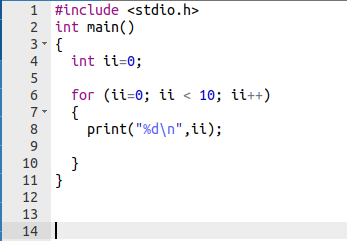
\includegraphics[scale=0.4]{../img/exported/for_code.png}
\caption{Estructura repetitiva for: ejemplo}
\end{figure}
\end{columns}



\end{frame}

\begin{frame}{Ciclo repetitivo for: anidacion}
\begin{itemize}
   \item[]<1-> Inicio del algoritmo

   \begin{itemize}
   		\item[]<2-> i=0 definicion de la variable control ciclo repetivivo I
   		\item[]<3-> j=0 definicion de la variable control ciclo repetivivo II
     	\item[]<4-> Para i=0 hasta N
     		\item[]<5-> \hspace{0.3in} Para j=0 hasta M
     		\item[]<6->  \hspace{0.5in} accion dentro del ciclo II
         	\item[]<7->  \hspace{0.5in} accion dentro del ciclo II
			\item[]<8->  \hspace{0.5in} accion dentro del ciclo II
   
   \item[]<9->  \hspace{0.3in}  accion dentro del ciclo I
   \item[]<10->  \hspace{0.3in}  accion dentro del ciclo I
   \item[]<11->  \hspace{0.3in}  accion dentro del ciclo I
   \end{itemize}
  \item[]<12-> Fin del algoritmo\end{itemize}
\end{frame}


\begin{frame}{Ciclo repetitivo for: anidacion}
\codesetstylefrombeamer
\cppfile{../../c/src/3-4-for.c}
\end{frame}




\begin{frame}{Ciclo repetitivo for: ejemplos}
 \begin{enumerate}
   
  \item Diseñar y codificar un programa en C que reciba 10 numeros ingresados por teclado e imprima la cantidad de positivos y negativos.El cero es considerado positivo.
\href{https://github.com/danis963/informaticaI_IUA/blob/main/c/src/3-2-for.c}{\beamergotobutton{Ver en github}}


  \item Diseñar y codificar un programa en C que reciba
la cantidad de filas y columnas de una matriz y luego imprima 
dicha matriz donde cada elemento vale la suma de su posicion en filas y columnas
\href{https://github.com/danis963/informaticaI_IUA/blob/main/c/src/3-5-for.c}{\beamergotobutton{Ver en github}}

   \end{enumerate}
   

\end{frame}
\end{document}